\documentclass{article}
\usepackage{graphicx}
\usepackage{float}
\usepackage{xcolor}
\usepackage{listings}

\definecolor{lightgray}{rgb}{.9,.9,.9}
\definecolor{darkgray}{rgb}{.4,.4,.4}
\definecolor{purple}{rgb}{0.65, 0.12, 0.82}

\lstdefinelanguage{JavaScript}{
  keywords={message, const, typeof, new, true, false, catch, function, return, null, catch, switch, var, if, in, while, do, else, case, break},
  keywordstyle=\color{blue}\bfseries,
  ndkeywords={class, export, boolean, throw, implements, import, this},
  ndkeywordstyle=\color{darkgray}\bfseries,
  identifierstyle=\color{black},
  sensitive=false,
  comment=[l]{//},
  morecomment=[s]{/*}{*/},
  commentstyle=\color{purple}\ttfamily,
  stringstyle=\color{red}\ttfamily,
  morestring=[b]',
  morestring=[b]"
}

\lstset{
   language=JavaScript,
   backgroundcolor=\color{lightgray},
   extendedchars=true,
   basicstyle=\footnotesize\ttfamily,
   showstringspaces=false,
   showspaces=false,
   numbers=left,
   numberstyle=\footnotesize,
   numbersep=9pt,
   tabsize=2,
   breaklines=true,
   showtabs=false,
   captionpos=b
}

\title{Final Project: Hybrid centralized and p2p chat system SOCKET}
\date{16/4/2020}
\author{Distributed System Group 4}

\begin{document}
\maketitle
\pagenumbering{gobble}
\newpage
\tableofcontents
\newpage
\pagenumbering{arabic}


\section{Introduction}
\paragraph{}
Like many great chefs who like to cook their own foods. We as a programmers, who also likes to build our own application, because we can have absolute control to add and remove things we like and dislike while also have better privacy.
\paragraph{}
Although we cannot replace anything and everything, and we also don't have the knowledge or resource required to do so alone. We could, however, build a simple small-scaled application for the sake of gaining experience and deeper understanding of the technology rather than to replace what other people have made very well.
\paragraph{}
So with the help of Dr Son and what we have learned in the Distributed System course, we took on the challenge to make a p2p chat system, and in this report we will detain How we design and build the system, What tools did we use, And what we have accomplished.

\section{Model}
\paragraph{Basic flow}
When a new client connects to the server. The server will tell existing clients to connect with the new client, forming p2p connection. Also, same thing applied when the server tells other clients that a client has disconnected, or terminated.
    \begin{figure}[H]
    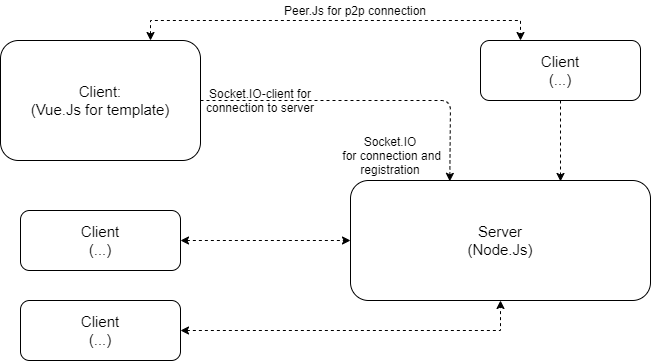
\includegraphics[width=\linewidth]{Model.png}
    \caption{Model}
    \end{figure}

\section{Tools}
\subsection{PeerJS}
    \paragraph{Definition}    
    PeerJS simplifies peer-to-peer data, video, and audio calls.
    \paragraph{Usage}
    Every Peer object is assigned a random, unique ID when it's created.

    \begin{lstlisting}
    peer.on('open', function(id) {
    console.log('My peer ID is: ' + id);
    });
    \end{lstlisting}

     When we want to connect to another peer, we'll need to know their peer id. You're in charge of communicating the peer IDs between users of your site.
    
    \paragraph{Data connection}
    Start a data connection by calling peer.connect with the peer ID of the destination peer.

    \begin{lstlisting}[caption = Start connection ]
        var conn = peer.connect('dest-peer-id');
    \end{lstlisting}

    \begin{lstlisting}[caption = Receive connection ]
        peer.on('connection', function(conn) { ... });
    \end{lstlisting}

    Anytime another peer attempts to connect to your peer ID, you'll receive a connection event.
    peer.connect and the callback of the connection event will both provide a DataConnection object. This object will allow you to send and receive data:

    \begin{lstlisting}
        conn.on('open', function() {
            // Receive messages
            conn.on('data', function(data) {
            console.log('Received', data);
            });
        
            // Send messages
            conn.send('Hello!');
        });
    \end{lstlisting}

    \paragraph{What kind of data can I send?}
    PeerJS has the BinaryPack serialization format built-in. This means you can send any JSON type as well as binary Blobs and ArrayBuffers. Simply send arbitrary data and you'll get it out the other side:

    \begin{lstlisting}
        conn.send({
            strings: 'hi!',
            numbers: 150,
            arrays: [1,2,3],
            evenBinary: new Blob([1,2,3]),
            andMore: {bool: true}
          });
    \end{lstlisting}



    \paragraph{What about latency/bandwidth?}
    Data sent between the two peers do not touch any other servers, so the connection speed is limited only by the upload and download rates of the two peers. This also means you don't have the additional latency of an intermediary server.
    \newline
    The latency to establish a connection can be split into two components: the brokering of data and the identification of clients. PeerJS has been designed to minimize the time you spend in these two areas. For brokering, data is sent through an XHR streaming request before a WebSocket connection is established, then through WebSockets. For client identification, we provide you the ability to pass in your own peer IDs, thus eliminating the RTT for retrieving an ID from the server.

\subsection{SocketIO}
\paragraph{Definition} 
Socket.IO is a library that enables real-time, bidirectional and event-based communication between the browser and the server. It consists of:

\begin{itemize}
	\item a Node.js server
	\item a Javascript client library for the browser (which can be also run from Node.js)
\end{itemize}

\paragraph{Its main features are:}
\subparagraph{Reliability}
Connections are established even in the presence of:
proxies and load balancers.
personal firewall and antivirus software.
For this purpose, it relies on Engine.IO, which first establishes a long-polling connection, then tries to upgrade to better transports that are “tested” on the side, like WebSocket. Please see the Goals section for more information.

\subsection{VueJS}
\paragraph{}
Vue is a progressive framework for building user interfaces. Unlike other monolithic frameworks, Vue is designed from the ground up to be incrementally adoptable. The core library is focused on the view layer only, and is easy to pick up and integrate with other libraries or existing projects. On the other hand, Vue is also perfectly capable of powering sophisticated Single-Page Applications when used in combination with modern tooling and supporting libraries.


\section{Conclusion}
\subsection{Write new users to the database}
\subsection{Event listenner}





\section{Who does what?}

\begin{itemize}
	\item Bui Quang Huy
	\item Nguyen Viet Dung
	\item Nguyen Quang Trung
	\item Do Minh Hoang
	\item Pham Minh kien
\end{itemize}

\end{document}